% Options for packages loaded elsewhere
\PassOptionsToPackage{unicode}{hyperref}
\PassOptionsToPackage{hyphens}{url}
\PassOptionsToPackage{dvipsnames,svgnames,x11names}{xcolor}
%
\documentclass[
  letterpaper,
  DIV=11,
  numbers=noendperiod]{scrreprt}

\usepackage{amsmath,amssymb}
\usepackage{lmodern}
\usepackage{iftex}
\ifPDFTeX
  \usepackage[T1]{fontenc}
  \usepackage[utf8]{inputenc}
  \usepackage{textcomp} % provide euro and other symbols
\else % if luatex or xetex
  \usepackage{unicode-math}
  \defaultfontfeatures{Scale=MatchLowercase}
  \defaultfontfeatures[\rmfamily]{Ligatures=TeX,Scale=1}
\fi
% Use upquote if available, for straight quotes in verbatim environments
\IfFileExists{upquote.sty}{\usepackage{upquote}}{}
\IfFileExists{microtype.sty}{% use microtype if available
  \usepackage[]{microtype}
  \UseMicrotypeSet[protrusion]{basicmath} % disable protrusion for tt fonts
}{}
\makeatletter
\@ifundefined{KOMAClassName}{% if non-KOMA class
  \IfFileExists{parskip.sty}{%
    \usepackage{parskip}
  }{% else
    \setlength{\parindent}{0pt}
    \setlength{\parskip}{6pt plus 2pt minus 1pt}}
}{% if KOMA class
  \KOMAoptions{parskip=half}}
\makeatother
\usepackage{xcolor}
\setlength{\emergencystretch}{3em} % prevent overfull lines
\setcounter{secnumdepth}{-\maxdimen} % remove section numbering
% Make \paragraph and \subparagraph free-standing
\ifx\paragraph\undefined\else
  \let\oldparagraph\paragraph
  \renewcommand{\paragraph}[1]{\oldparagraph{#1}\mbox{}}
\fi
\ifx\subparagraph\undefined\else
  \let\oldsubparagraph\subparagraph
  \renewcommand{\subparagraph}[1]{\oldsubparagraph{#1}\mbox{}}
\fi

\usepackage{color}
\usepackage{fancyvrb}
\newcommand{\VerbBar}{|}
\newcommand{\VERB}{\Verb[commandchars=\\\{\}]}
\DefineVerbatimEnvironment{Highlighting}{Verbatim}{commandchars=\\\{\}}
% Add ',fontsize=\small' for more characters per line
\usepackage{framed}
\definecolor{shadecolor}{RGB}{241,243,245}
\newenvironment{Shaded}{\begin{snugshade}}{\end{snugshade}}
\newcommand{\AlertTok}[1]{\textcolor[rgb]{0.68,0.00,0.00}{#1}}
\newcommand{\AnnotationTok}[1]{\textcolor[rgb]{0.37,0.37,0.37}{#1}}
\newcommand{\AttributeTok}[1]{\textcolor[rgb]{0.40,0.45,0.13}{#1}}
\newcommand{\BaseNTok}[1]{\textcolor[rgb]{0.68,0.00,0.00}{#1}}
\newcommand{\BuiltInTok}[1]{\textcolor[rgb]{0.00,0.23,0.31}{#1}}
\newcommand{\CharTok}[1]{\textcolor[rgb]{0.13,0.47,0.30}{#1}}
\newcommand{\CommentTok}[1]{\textcolor[rgb]{0.37,0.37,0.37}{#1}}
\newcommand{\CommentVarTok}[1]{\textcolor[rgb]{0.37,0.37,0.37}{\textit{#1}}}
\newcommand{\ConstantTok}[1]{\textcolor[rgb]{0.56,0.35,0.01}{#1}}
\newcommand{\ControlFlowTok}[1]{\textcolor[rgb]{0.00,0.23,0.31}{#1}}
\newcommand{\DataTypeTok}[1]{\textcolor[rgb]{0.68,0.00,0.00}{#1}}
\newcommand{\DecValTok}[1]{\textcolor[rgb]{0.68,0.00,0.00}{#1}}
\newcommand{\DocumentationTok}[1]{\textcolor[rgb]{0.37,0.37,0.37}{\textit{#1}}}
\newcommand{\ErrorTok}[1]{\textcolor[rgb]{0.68,0.00,0.00}{#1}}
\newcommand{\ExtensionTok}[1]{\textcolor[rgb]{0.00,0.23,0.31}{#1}}
\newcommand{\FloatTok}[1]{\textcolor[rgb]{0.68,0.00,0.00}{#1}}
\newcommand{\FunctionTok}[1]{\textcolor[rgb]{0.28,0.35,0.67}{#1}}
\newcommand{\ImportTok}[1]{\textcolor[rgb]{0.00,0.46,0.62}{#1}}
\newcommand{\InformationTok}[1]{\textcolor[rgb]{0.37,0.37,0.37}{#1}}
\newcommand{\KeywordTok}[1]{\textcolor[rgb]{0.00,0.23,0.31}{#1}}
\newcommand{\NormalTok}[1]{\textcolor[rgb]{0.00,0.23,0.31}{#1}}
\newcommand{\OperatorTok}[1]{\textcolor[rgb]{0.37,0.37,0.37}{#1}}
\newcommand{\OtherTok}[1]{\textcolor[rgb]{0.00,0.23,0.31}{#1}}
\newcommand{\PreprocessorTok}[1]{\textcolor[rgb]{0.68,0.00,0.00}{#1}}
\newcommand{\RegionMarkerTok}[1]{\textcolor[rgb]{0.00,0.23,0.31}{#1}}
\newcommand{\SpecialCharTok}[1]{\textcolor[rgb]{0.37,0.37,0.37}{#1}}
\newcommand{\SpecialStringTok}[1]{\textcolor[rgb]{0.13,0.47,0.30}{#1}}
\newcommand{\StringTok}[1]{\textcolor[rgb]{0.13,0.47,0.30}{#1}}
\newcommand{\VariableTok}[1]{\textcolor[rgb]{0.07,0.07,0.07}{#1}}
\newcommand{\VerbatimStringTok}[1]{\textcolor[rgb]{0.13,0.47,0.30}{#1}}
\newcommand{\WarningTok}[1]{\textcolor[rgb]{0.37,0.37,0.37}{\textit{#1}}}

\providecommand{\tightlist}{%
  \setlength{\itemsep}{0pt}\setlength{\parskip}{0pt}}\usepackage{longtable,booktabs,array}
\usepackage{calc} % for calculating minipage widths
% Correct order of tables after \paragraph or \subparagraph
\usepackage{etoolbox}
\makeatletter
\patchcmd\longtable{\par}{\if@noskipsec\mbox{}\fi\par}{}{}
\makeatother
% Allow footnotes in longtable head/foot
\IfFileExists{footnotehyper.sty}{\usepackage{footnotehyper}}{\usepackage{footnote}}
\makesavenoteenv{longtable}
\usepackage{graphicx}
\makeatletter
\def\maxwidth{\ifdim\Gin@nat@width>\linewidth\linewidth\else\Gin@nat@width\fi}
\def\maxheight{\ifdim\Gin@nat@height>\textheight\textheight\else\Gin@nat@height\fi}
\makeatother
% Scale images if necessary, so that they will not overflow the page
% margins by default, and it is still possible to overwrite the defaults
% using explicit options in \includegraphics[width, height, ...]{}
\setkeys{Gin}{width=\maxwidth,height=\maxheight,keepaspectratio}
% Set default figure placement to htbp
\makeatletter
\def\fps@figure{htbp}
\makeatother

\KOMAoption{captions}{tableheading}
\makeatletter
\makeatother
\makeatletter
\makeatother
\makeatletter
\@ifpackageloaded{caption}{}{\usepackage{caption}}
\AtBeginDocument{%
\ifdefined\contentsname
  \renewcommand*\contentsname{Table of contents}
\else
  \newcommand\contentsname{Table of contents}
\fi
\ifdefined\listfigurename
  \renewcommand*\listfigurename{List of Figures}
\else
  \newcommand\listfigurename{List of Figures}
\fi
\ifdefined\listtablename
  \renewcommand*\listtablename{List of Tables}
\else
  \newcommand\listtablename{List of Tables}
\fi
\ifdefined\figurename
  \renewcommand*\figurename{Figure}
\else
  \newcommand\figurename{Figure}
\fi
\ifdefined\tablename
  \renewcommand*\tablename{Table}
\else
  \newcommand\tablename{Table}
\fi
}
\@ifpackageloaded{float}{}{\usepackage{float}}
\floatstyle{ruled}
\@ifundefined{c@chapter}{\newfloat{codelisting}{h}{lop}}{\newfloat{codelisting}{h}{lop}[chapter]}
\floatname{codelisting}{Listing}
\newcommand*\listoflistings{\listof{codelisting}{List of Listings}}
\makeatother
\makeatletter
\@ifpackageloaded{caption}{}{\usepackage{caption}}
\@ifpackageloaded{subcaption}{}{\usepackage{subcaption}}
\makeatother
\makeatletter
\@ifpackageloaded{tcolorbox}{}{\usepackage[many]{tcolorbox}}
\makeatother
\makeatletter
\@ifundefined{shadecolor}{\definecolor{shadecolor}{rgb}{.97, .97, .97}}
\makeatother
\makeatletter
\makeatother
\ifLuaTeX
  \usepackage{selnolig}  % disable illegal ligatures
\fi
\IfFileExists{bookmark.sty}{\usepackage{bookmark}}{\usepackage{hyperref}}
\IfFileExists{xurl.sty}{\usepackage{xurl}}{} % add URL line breaks if available
\urlstyle{same} % disable monospaced font for URLs
\hypersetup{
  colorlinks=true,
  linkcolor={blue},
  filecolor={Maroon},
  citecolor={Blue},
  urlcolor={Blue},
  pdfcreator={LaTeX via pandoc}}

\author{}
\date{}

\begin{document}
\ifdefined\Shaded\renewenvironment{Shaded}{\begin{tcolorbox}[boxrule=0pt, sharp corners, enhanced, borderline west={3pt}{0pt}{shadecolor}, frame hidden, interior hidden, breakable]}{\end{tcolorbox}}\fi

\hypertarget{analysis}{%
\chapter{Analysis}\label{analysis}}

\hypertarget{visualization}{%
\section{Visualization}\label{visualization}}

\begin{Shaded}
\begin{Highlighting}[]
\NormalTok{df }\OtherTok{\textless{}{-}} \FunctionTok{read.csv}\NormalTok{(}\StringTok{"TrainData.csv"}\NormalTok{) }\SpecialCharTok{|\textgreater{}}
  \FunctionTok{na.omit}\NormalTok{() }\SpecialCharTok{|\textgreater{}}
  \FunctionTok{distinct}\NormalTok{()}

\CommentTok{\# head(df2)}
\CommentTok{\# colnames(df2)}
\end{Highlighting}
\end{Shaded}

\hypertarget{visualizing-quantile-regression-vs-ols}{%
\subsection{Visualizing quantile regression vs
OLS}\label{visualizing-quantile-regression-vs-ols}}

\begin{Shaded}
\begin{Highlighting}[]
\NormalTok{df }\SpecialCharTok{|\textgreater{}} \FunctionTok{ggplot}\NormalTok{(}\FunctionTok{aes}\NormalTok{(}\AttributeTok{y =}\NormalTok{ SalePrice, }\AttributeTok{x =}\NormalTok{ LotArea)) }\SpecialCharTok{+}
  \FunctionTok{geom\_point}\NormalTok{(}\AttributeTok{size =} \FloatTok{0.9}\NormalTok{) }\SpecialCharTok{+}
  \FunctionTok{geom\_smooth}\NormalTok{(}\AttributeTok{method =}\NormalTok{ lm, }\AttributeTok{se =}\NormalTok{ F, }\AttributeTok{color =} \StringTok{"black"}\NormalTok{) }\SpecialCharTok{+}
  \FunctionTok{geom\_text}\NormalTok{(}\FunctionTok{aes}\NormalTok{(}\AttributeTok{y =} \DecValTok{400000}\NormalTok{, }\AttributeTok{x =} \DecValTok{150000}\NormalTok{, }\AttributeTok{label =} \StringTok{"OLS"}\NormalTok{), }\AttributeTok{color=}\StringTok{"black"}\NormalTok{) }\SpecialCharTok{+} 
  \FunctionTok{geom\_quantile}\NormalTok{(}\AttributeTok{quantiles=}\FloatTok{0.5}\NormalTok{, }\AttributeTok{color=}\StringTok{"red"}\NormalTok{) }\SpecialCharTok{+} 
  \FunctionTok{geom\_text}\NormalTok{(}\FunctionTok{aes}\NormalTok{(}\AttributeTok{y =} \DecValTok{470000}\NormalTok{, }\AttributeTok{x =} \DecValTok{90000}\NormalTok{, }\AttributeTok{label =} \StringTok{"50th quantile"}\NormalTok{), }\AttributeTok{color=}\StringTok{"red"}\NormalTok{) }\SpecialCharTok{+} 
  \FunctionTok{ylab}\NormalTok{(}\StringTok{"Sale price ($)"}\NormalTok{) }\SpecialCharTok{+}
  \FunctionTok{xlab}\NormalTok{(}\StringTok{"Lot area (Square feet)"}\NormalTok{) }\SpecialCharTok{+}
  \FunctionTok{theme\_bw}\NormalTok{()}
\end{Highlighting}
\end{Shaded}

\begin{verbatim}
`geom_smooth()` using formula = 'y ~ x'
Smoothing formula not specified. Using: y ~ x
\end{verbatim}

\begin{figure}[H]

{\centering 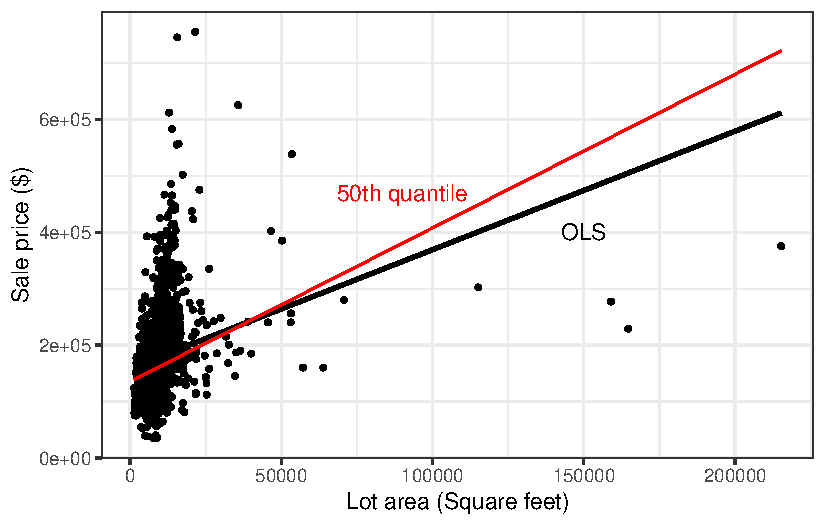
\includegraphics{analysis_files/figure-pdf/Visualizing housing-1.pdf}

}

\end{figure}

\begin{Shaded}
\begin{Highlighting}[]
\NormalTok{df }\SpecialCharTok{|\textgreater{}} \FunctionTok{ggplot}\NormalTok{(}\FunctionTok{aes}\NormalTok{(}\AttributeTok{y =}\NormalTok{ SalePrice, }\AttributeTok{x =}\NormalTok{ GrLivArea)) }\SpecialCharTok{+}
  \FunctionTok{geom\_point}\NormalTok{(}\AttributeTok{size =} \FloatTok{0.9}\NormalTok{) }\SpecialCharTok{+}
  \FunctionTok{stat\_smooth}\NormalTok{(}\AttributeTok{method =}\NormalTok{ lm, }\AttributeTok{color =} \StringTok{"black"}\NormalTok{) }\SpecialCharTok{+}
  \FunctionTok{geom\_text}\NormalTok{(}\FunctionTok{aes}\NormalTok{(}\AttributeTok{x =} \DecValTok{4150}\NormalTok{, }\AttributeTok{y =} \DecValTok{500000}\NormalTok{, }\AttributeTok{label =} \StringTok{"OLS"}\NormalTok{), }\AttributeTok{color=}\StringTok{"black"}\NormalTok{) }\SpecialCharTok{+} 
  \FunctionTok{geom\_quantile}\NormalTok{(}\AttributeTok{quantiles=}\FloatTok{0.25}\NormalTok{, }\AttributeTok{color=}\StringTok{"red"}\NormalTok{) }\SpecialCharTok{+} 
  \FunctionTok{geom\_text}\NormalTok{(}\FunctionTok{aes}\NormalTok{(}\AttributeTok{x =} \DecValTok{4000}\NormalTok{, }\AttributeTok{y =} \DecValTok{270000}\NormalTok{, }\AttributeTok{label =} \StringTok{"25th quantile"}\NormalTok{), }\AttributeTok{color=}\StringTok{"red"}\NormalTok{) }\SpecialCharTok{+} 
  \FunctionTok{geom\_quantile}\NormalTok{(}\AttributeTok{quantiles=}\FloatTok{0.5}\NormalTok{, }\AttributeTok{color=}\StringTok{"blue"}\NormalTok{) }\SpecialCharTok{+} 
  \FunctionTok{geom\_text}\NormalTok{(}\FunctionTok{aes}\NormalTok{(}\AttributeTok{x =} \DecValTok{4150}\NormalTok{, }\AttributeTok{y =} \DecValTok{400000}\NormalTok{, }\AttributeTok{label =} \StringTok{"50th"}\NormalTok{), }\AttributeTok{color=}\StringTok{"blue"}\NormalTok{) }\SpecialCharTok{+} 
  \FunctionTok{geom\_quantile}\NormalTok{(}\AttributeTok{quantiles=}\FloatTok{0.75}\NormalTok{, }\AttributeTok{color=}\StringTok{"green"}\NormalTok{) }\SpecialCharTok{+} 
  \FunctionTok{geom\_text}\NormalTok{(}\FunctionTok{aes}\NormalTok{(}\AttributeTok{x =} \DecValTok{4000}\NormalTok{, }\AttributeTok{y =} \DecValTok{600000}\NormalTok{, }\AttributeTok{label =} \StringTok{"75th quantile"}\NormalTok{), }\AttributeTok{color=}\StringTok{"green"}\NormalTok{) }\SpecialCharTok{+} 
  \FunctionTok{xlab}\NormalTok{(}\StringTok{"Sale price ($)"}\NormalTok{) }\SpecialCharTok{+}
  \FunctionTok{ylab}\NormalTok{(}\StringTok{"Above ground area (Square feet)"}\NormalTok{) }\SpecialCharTok{+}
  \FunctionTok{theme\_bw}\NormalTok{()}
\end{Highlighting}
\end{Shaded}

\begin{verbatim}
`geom_smooth()` using formula = 'y ~ x'
Smoothing formula not specified. Using: y ~ x
Smoothing formula not specified. Using: y ~ x
Smoothing formula not specified. Using: y ~ x
\end{verbatim}

\begin{figure}[H]

{\centering 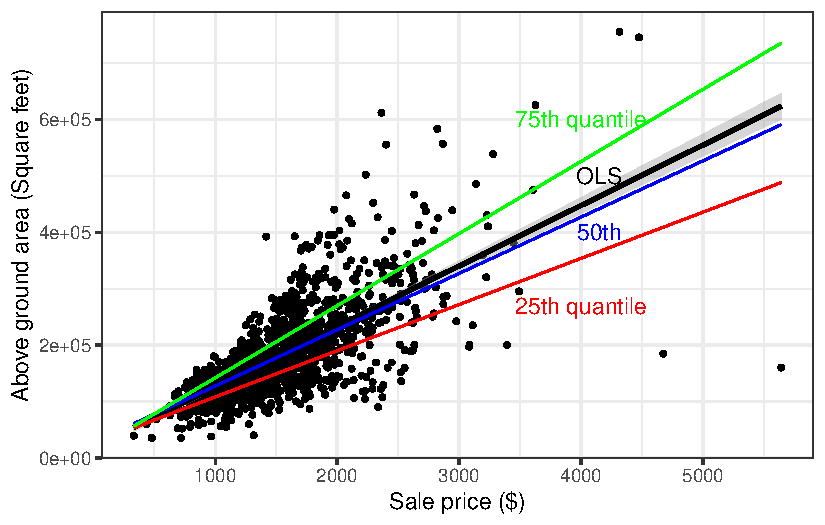
\includegraphics{analysis_files/figure-pdf/Visualizing housing-2.pdf}

}

\end{figure}

\hypertarget{model-creation}{%
\section{Model creation}\label{model-creation}}

\hypertarget{qr-model}{%
\subsection{QR model}\label{qr-model}}

\begin{Shaded}
\begin{Highlighting}[]
\NormalTok{qreg\_model50 }\OtherTok{=} \FunctionTok{rq}\NormalTok{(}\AttributeTok{data=}\NormalTok{df, SalePrice }\SpecialCharTok{\textasciitilde{}}\NormalTok{ GrLivArea }\SpecialCharTok{+}\NormalTok{ LotArea }\SpecialCharTok{+}\NormalTok{ TotRmsAbvGrd }\SpecialCharTok{+} \FunctionTok{as.factor}\NormalTok{(LotShape) }\SpecialCharTok{+} \FunctionTok{as.factor}\NormalTok{(Foundation), }\AttributeTok{tau=}\FloatTok{0.5}\NormalTok{)}
\end{Highlighting}
\end{Shaded}

\begin{verbatim}
Warning in rq.fit.br(x, y, tau = tau, ...): Solution may be nonunique
\end{verbatim}

\begin{Shaded}
\begin{Highlighting}[]
\FunctionTok{summary}\NormalTok{(qreg\_model50)}
\end{Highlighting}
\end{Shaded}

\begin{verbatim}
Warning in summary.rq(qreg_model50): 3 non-positive fis
\end{verbatim}

\begin{verbatim}

Call: rq(formula = SalePrice ~ GrLivArea + LotArea + TotRmsAbvGrd + 
    as.factor(LotShape) + as.factor(Foundation), tau = 0.5, data = df)

tau: [1] 0.5

Coefficients:
                            Value        Std. Error   t value      Pr(>|t|)    
(Intercept)                  36326.81296   3853.84854      9.42611      0.00000
GrLivArea                       96.66934      4.02708     24.00481      0.00000
LotArea                          0.99940      0.32815      3.04561      0.00236
TotRmsAbvGrd                 -6476.18114   1080.95132     -5.99119      0.00000
as.factor(LotShape)IR2       -5084.13375   7841.20685     -0.64839      0.51684
as.factor(LotShape)IR3      -21074.80675   7616.42154     -2.76702      0.00573
as.factor(LotShape)Reg      -11065.07360   2020.92512     -5.47525      0.00000
as.factor(Foundation)CBlock  21252.40678   1709.40460     12.43264      0.00000
as.factor(Foundation)PConc   53311.16094   2618.05941     20.36285      0.00000
as.factor(Foundation)Slab   -16867.20619   5378.30454     -3.13616      0.00175
as.factor(Foundation)Stone   14561.54748  13561.64146      1.07373      0.28312
as.factor(Foundation)Wood    -2008.81877   9022.14216     -0.22265      0.82384
\end{verbatim}

\hypertarget{ols-model}{%
\subsection{OLS model}\label{ols-model}}

\begin{Shaded}
\begin{Highlighting}[]
\NormalTok{ols }\OtherTok{=} \FunctionTok{lm}\NormalTok{(}\AttributeTok{data=}\NormalTok{df, SalePrice }\SpecialCharTok{\textasciitilde{}}\NormalTok{ GrLivArea }\SpecialCharTok{+}\NormalTok{ LotArea }\SpecialCharTok{+}\NormalTok{ TotRmsAbvGrd }\SpecialCharTok{+} \FunctionTok{as.factor}\NormalTok{(LotShape) }\SpecialCharTok{+} \FunctionTok{as.factor}\NormalTok{(Foundation))}
\FunctionTok{summary}\NormalTok{(ols)}
\end{Highlighting}
\end{Shaded}

\begin{verbatim}

Call:
lm(formula = SalePrice ~ GrLivArea + LotArea + TotRmsAbvGrd + 
    as.factor(LotShape) + as.factor(Foundation), data = df)

Residuals:
    Min      1Q  Median      3Q     Max 
-422488  -26194    -805   20461  326538 

Coefficients:
                              Estimate Std. Error t value Pr(>|t|)    
(Intercept)                  2.005e+04  7.267e+03   2.759  0.00587 ** 
GrLivArea                    9.893e+01  4.538e+00  21.801  < 2e-16 ***
LotArea                      9.173e-01  1.425e-01   6.438 1.64e-10 ***
TotRmsAbvGrd                -4.313e+03  1.396e+03  -3.089  0.00205 ** 
as.factor(LotShape)IR2      -2.009e+03  8.113e+03  -0.248  0.80446    
as.factor(LotShape)IR3      -6.936e+04  1.603e+04  -4.328 1.61e-05 ***
as.factor(LotShape)Reg      -1.342e+04  2.809e+03  -4.777 1.96e-06 ***
as.factor(Foundation)CBlock  2.094e+04  4.497e+03   4.656 3.52e-06 ***
as.factor(Foundation)PConc   6.679e+04  4.541e+03  14.708  < 2e-16 ***
as.factor(Foundation)Slab   -1.426e+04  1.067e+04  -1.336  0.18170    
as.factor(Foundation)Stone  -3.396e+03  2.021e+04  -0.168  0.86658    
as.factor(Foundation)Wood   -5.553e+02  2.842e+04  -0.020  0.98441    
---
Signif. codes:  0 '***' 0.001 '**' 0.01 '*' 0.05 '.' 0.1 ' ' 1

Residual standard error: 48410 on 1448 degrees of freedom
Multiple R-squared:  0.6315,    Adjusted R-squared:  0.6287 
F-statistic: 225.6 on 11 and 1448 DF,  p-value: < 2.2e-16
\end{verbatim}

\hypertarget{model-evaluation}{%
\section{Model evaluation}\label{model-evaluation}}

\hypertarget{mean-absolute-error}{%
\subsection{Mean absolute error}\label{mean-absolute-error}}

\hypertarget{root-mean-squared-error}{%
\subsection{Root mean squared error}\label{root-mean-squared-error}}

\hypertarget{variance-of-error}{%
\subsection{Variance of error}\label{variance-of-error}}

\hypertarget{minmax-error}{%
\subsection{Min/max error}\label{minmax-error}}



\end{document}
